\section{Installation and Deployment Guide}
\label{app:installation-guide}

This appendix provides comprehensive installation and deployment instructions for the Robotic Ultrasound System (RUS). The guide covers hardware setup, software installation, system configuration, and initial commissioning procedures.

\subsection{Pre-Installation Requirements}

\subsubsection{Site Preparation Checklist}

\begin{table}[htbp]
\centering
\caption{Site Preparation Requirements}
\label{tab:app-site-requirements}
\begin{tabular}{|l|l|c|}
\hline
\textbf{Requirement} & \textbf{Specification} & \textbf{Verified} \\
\hline
Room Dimensions & Minimum 4m $\times$ 4m $\times$ 3m (W$\times$L$\times$H) & $\square$ \\
Floor Load Capacity & 2000 kg/m² & $\square$ \\
Power Supply & 230V $\pm$ 10\%, 50/60 Hz, 32A & $\square$ \\
UPS Backup & 30 minutes minimum runtime & $\square$ \\
Network Infrastructure & Gigabit Ethernet, isolated VLAN & $\square$ \\
Temperature Control & 18-25$^\circ$C (64-77$^\circ$F) & $\square$ \\
Humidity Control & 30-70\% RH, non-condensing & $\square$ \\
Vibration Isolation & $< 0.1$ mm/s RMS & $\square$ \\
EMI Shielding & Medical grade EMC protection & $\square$ \\
Emergency Stop Access & Within 3 meters of robot workspace & $\square$ \\
\hline
\end{tabular}
\end{table}

\subsubsection{Required Tools and Equipment}

\begin{lstlisting}[basicstyle=\ttfamily\footnotesize, caption={Installation Tool List}, label={lst:app-tools}]
REQUIRED TOOLS AND EQUIPMENT FOR RUS INSTALLATION

MECHANICAL TOOLS:
\checkmark Precision torque wrench set (5-200 Nm)
\checkmark Hex key set (metric, 2-20 mm)
\checkmark Socket wrench set (8-32 mm)
\checkmark Digital calipers (0.01 mm precision)
\checkmark Dial indicators and magnetic bases
\checkmark Spirit level (1 mm/m accuracy)
\checkmark Coordinate measuring machine (CMM) or laser tracker
\checkmark Mechanical lifting equipment (500 kg capacity)

ELECTRICAL TOOLS:
\checkmark Digital multimeter (true RMS)
\checkmark Oscilloscope (100 MHz minimum)
\checkmark Ground resistance tester
\checkmark Insulation resistance tester
\checkmark Power quality analyzer
\checkmark Cable management tools
\checkmark Crimp tools for various connectors
\checkmark Heat shrink tubing and heat gun

SOFTWARE TOOLS:
\checkmark Laptop with Windows 10/11 Pro or Ubuntu 20.04 LTS
\checkmark RUS Installation Software Package v2.1.0
\checkmark Network analyzer software
\checkmark Terminal emulation software
\checkmark System monitoring utilities
\checkmark Backup and imaging software

CALIBRATION EQUIPMENT:
\checkmark Certified force/torque sensors
\checkmark Precision position measurement system
\checkmark Ultrasound test phantoms
\checkmark Calibrated pressure sensors
\checkmark Temperature and humidity loggers
\checkmark Noise level meter

SAFETY EQUIPMENT:
\checkmark Personal protective equipment (PPE)
\checkmark Lockout/tagout (LOTO) devices
\checkmark Emergency stop test equipment
\checkmark First aid kit
\checkmark Fire extinguisher (Class C electrical)
\checkmark Spill containment materials

DOCUMENTATION:
\checkmark Installation checklist (this document)
\checkmark System specifications
\checkmark Electrical schematics
\checkmark Mechanical drawings
\checkmark Calibration certificates
\checkmark Test procedures and protocols
\end{lstlisting}

\subsection{Hardware Installation}

\subsubsection{Mechanical Assembly Procedure}

\begin{lstlisting}[basicstyle=\ttfamily\footnotesize, caption={Step-by-Step Mechanical Assembly}, label={lst:app-mechanical}]
MECHANICAL ASSEMBLY PROCEDURE
RUS System Hardware Installation

SAFETY NOTICE: 
Ensure all power is disconnected and locked out before beginning assembly.
Use appropriate lifting equipment for components over 25 kg.

STEP 1: BASE PLATFORM INSTALLATION (60 minutes)
1.1 Unpack base platform from shipping container
1.2 Inspect for shipping damage - document any issues
1.3 Position base platform using overhead crane/forklift
1.4 Level platform using adjustable feet
    - Target: $\pm$0.1 mm/m over entire surface
    - Use precision spirit level for verification
1.5 Anchor platform to floor using M16 anchor bolts
    - Torque specification: 150 $\pm$ 10 Nm
1.6 Connect grounding strap to facility earth ground
1.7 Verify platform stability - no movement under 100 kg load

STEP 2: ROBOT ARM MOUNTING (90 minutes)
2.1 Remove robot arm from shipping container using proper lifting
2.2 Inspect joint seals and protective covers
2.3 Mount robot base to platform flange
    - Use lifting fixture RUS-LF-001
    - Torque M12 bolts to 85 $\pm$ 5 Nm in star pattern
2.4 Connect robot base grounding cable
2.5 Install joint position sensors
    - Calibrate absolute position encoders
    - Verify $\pm$0.1$^\circ$ accuracy at all joints
2.6 Install force/torque sensor at end-effector
    - Calibrate using certified reference loads
    - Verify $\pm$0.5% accuracy over full range

STEP 3: ULTRASOUND PROBE ASSEMBLY (45 minutes)
3.1 Mount ultrasound probe holder to end-effector
3.2 Install probe orientation mechanism
    - Verify $\pm$0.1$^\circ$ resolution
    - Test full range of motion
3.3 Connect probe signal cables through cable management
3.4 Install probe force sensors
    - Calibrate contact force measurement
    - Set safety limits: 0.5-10.0 N

STEP 4: CONTROL CABINET INSTALLATION (75 minutes)
4.1 Position control cabinet in designated location
4.2 Ensure minimum 500 mm clearance on all sides
4.3 Connect main power cable (qualified electrician required)
4.4 Install UPS system and verify backup operation
4.5 Connect control cables to robot base
    - Use shielded cables with proper grounding
    - Verify cable continuity and insulation
4.6 Install emergency stop circuit
    - Test emergency stop function
    - Verify < 500 ms stop time

STEP 5: SENSOR SYSTEM INSTALLATION (60 minutes)
5.1 Install workspace cameras
    - Mount stereo camera pair for 3D vision
    - Calibrate camera intrinsic/extrinsic parameters
5.2 Install proximity sensors
    - IR sensors for collision avoidance
    - Ultrasonic sensors for backup detection
5.3 Install environmental monitoring
    - Temperature sensors ($\pm$0.1$^\circ$C accuracy)
    - Humidity sensors ($\pm$2% RH accuracy)
5.4 Connect all sensor cables to control system

FINAL MECHANICAL VERIFICATION:
\checkmark All fasteners torqued to specification
\checkmark All grounding connections verified
\checkmark No mechanical interference in full range of motion
\checkmark Emergency stops function correctly
\checkmark All sensors reading within specification
\checkmark Documentation complete and signed off

QUALITY CHECKPOINT:
Inspector: _________________ Date: _________
Signature: _________________________________
\end{lstlisting}

\subsubsection{Electrical System Installation}

\begin{figure}[htbp]
\centering
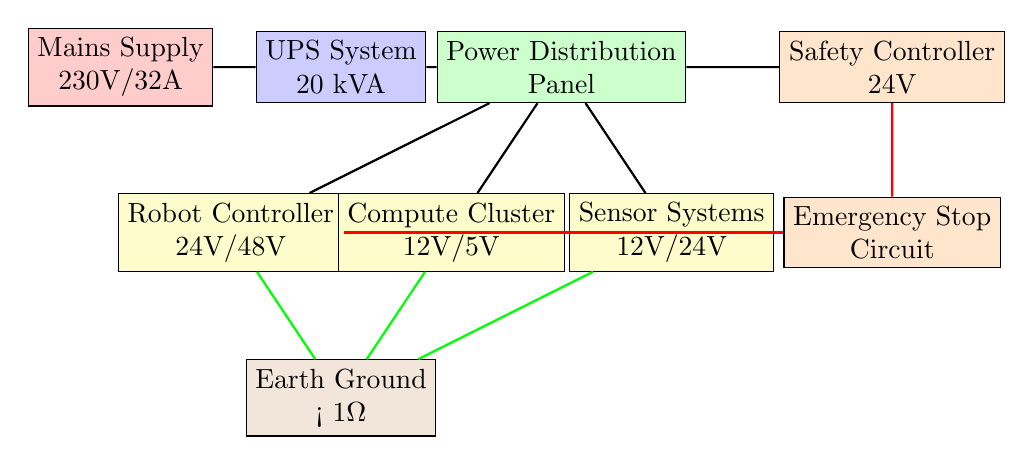
\begin{tikzpicture}[scale=0.7]
    % Main power distribution
    \node[draw, rectangle, fill=red!20, align=center] (mains) at (0,6) {Mains Supply\\230V/32A};
    \node[draw, rectangle, fill=blue!20, align=center] (ups) at (4,6) {UPS System\\20 kVA};
    \node[draw, rectangle, fill=green!20, align=center] (dist) at (8,6) {Power Distribution\\Panel};
    
    % Robot subsystems
    \node[draw, rectangle, fill=yellow!20, align=center] (robot) at (2,3) {Robot Controller\\24V/48V};
    \node[draw, rectangle, fill=yellow!20, align=center] (compute) at (6,3) {Compute Cluster\\12V/5V};
    \node[draw, rectangle, fill=yellow!20, align=center] (sensors) at (10,3) {Sensor Systems\\12V/24V};
    
    % Safety systems
    \node[draw, rectangle, fill=orange!20, align=center] (safety) at (14,6) {Safety Controller\\24V};
    \node[draw, rectangle, fill=orange!20, align=center] (estop) at (14,3) {Emergency Stop\\Circuit};
    
    % Connections
    \draw[thick] (mains) -- (ups);
    \draw[thick] (ups) -- (dist);
    \draw[thick] (dist) -- (safety);
    
    \draw[thick] (dist) -- (robot);
    \draw[thick] (dist) -- (compute);
    \draw[thick] (dist) -- (sensors);
    
    \draw[thick, red] (safety) -- (estop);
    \draw[thick, red] (estop) -- (robot);
    
    % Grounding
    \node[draw, rectangle, fill=brown!20, align=center] (ground) at (4,0) {Earth Ground\\< 1$\Omega$};
    \draw[thick, green] (robot) -- (ground);
    \draw[thick, green] (compute) -- (ground);
    \draw[thick, green] (sensors) -- (ground);
    
\end{tikzpicture}
\caption{Electrical System Architecture and Power Distribution}
\label{fig:app-electrical-system}
\end{figure}

\subsection{Software Installation}

\subsubsection{Operating System Setup}

\begin{lstlisting}[language=bash, caption={Operating System Installation Script}, label={lst:app-os-setup}]
#!/bin/bash
# RUS System Operating System Setup Script
# Version: 2.1.0
# Requires: Ubuntu 20.04 LTS with real-time kernel

set -e  # Exit on any error

echo "======================================"
echo "RUS System OS Setup v2.1.0"
echo "======================================"

# Verify system requirements
check_system_requirements() {
    echo "Checking system requirements..."
    
    # Check Ubuntu version
    if ! lsb_release -d | grep -q "Ubuntu 20.04"; then
        echo "ERROR: Ubuntu 20.04 LTS required"
        exit 1
    fi
    
    # Check architecture
    if [ "$(uname -m)" != "x86_64" ]; then
        echo "ERROR: x86_64 architecture required"
        exit 1
    fi
    
    # Check memory (minimum 16GB)
    total_mem=$(grep MemTotal /proc/meminfo | awk '{print $2}')
    if [ $total_mem -lt 16000000 ]; then
        echo "ERROR: Minimum 16GB RAM required"
        exit 1
    fi
    
    # Check CPU cores (minimum 8)
    cpu_cores=$(nproc)
    if [ $cpu_cores -lt 8 ]; then
        echo "ERROR: Minimum 8 CPU cores required"
        exit 1
    fi
    
    echo "System requirements satisfied"
}

# Install real-time kernel
install_rt_kernel() {
    echo "Installing real-time kernel..."
    
    sudo apt update
    sudo apt install -y linux-image-5.4.0-rt-amd64
    sudo apt install -y linux-headers-5.4.0-rt-amd64
    
    # Configure GRUB for RT kernel
    sudo sed -i 's/GRUB_DEFAULT=0/GRUB_DEFAULT="Advanced options for Ubuntu>Ubuntu, with Linux 5.4.0-rt-amd64"/' /etc/default/grub
    sudo update-grub
    
    echo "Real-time kernel installed. Reboot required."
}

# Configure real-time parameters
configure_rt_system() {
    echo "Configuring real-time system parameters..."
    
    # Set RT scheduling limits
    cat << EOF | sudo tee /etc/security/limits.d/99-rus-rt.conf
# RUS real-time limits
@rus-rt soft rtprio 99
@rus-rt hard rtprio 99
@rus-rt soft memlock unlimited
@rus-rt hard memlock unlimited
EOF
    
    # Create RUS RT group
    sudo groupadd -f rus-rt
    sudo usermod -a -G rus-rt $USER
    
    # Configure CPU isolation
    sudo sed -i 's/GRUB_CMDLINE_LINUX_DEFAULT="[^"]*/& isolcpus=2-7 nohz_full=2-7 rcu_nocbs=2-7/' /etc/default/grub
    sudo update-grub
    
    # Disable unnecessary services
    sudo systemctl disable bluetooth.service
    sudo systemctl disable cups.service
    sudo systemctl disable whoopsie.service
    sudo systemctl disable snapd.service
    
    echo "Real-time configuration complete"
}

# Install RUS dependencies
install_dependencies() {
    echo "Installing RUS system dependencies..."
    
    # Add RUS repository
    curl -fsSL https://packages.rus-medical.com/gpg | sudo apt-key add -
    echo "deb [arch=amd64] https://packages.rus-medical.com/ubuntu focal main" | sudo tee /etc/apt/sources.list.d/rus.list
    
    sudo apt update
    
    # Install core dependencies
    sudo apt install -y \
        build-essential \
        cmake \
        git \
        python3-dev \
        python3-pip \
        libboost-all-dev \
        libeigen3-dev \
        libopencv-dev \
        libpcl-dev \
        ros-noetic-desktop-full \
        xenomai-runtime \
        libxenomai-dev
    
    # Install Python packages
    pip3 install --user \
        numpy \
        scipy \
        matplotlib \
        scikit-learn \
        opencv-python \
        pyserial \
        psutil
    
    echo "Dependencies installed successfully"
}

# Configure network settings
configure_network() {
    echo "Configuring network settings..."
    
    # Create RUS network configuration
    cat << EOF | sudo tee /etc/netplan/99-rus-network.yaml
network:
  version: 2
  ethernets:
    rus-control:
      match:
        name: enp*s0
      addresses:
        - 192.168.100.10/24
      nameservers:
        addresses: [8.8.8.8, 8.8.4.4]
      routes:
        - to: 0.0.0.0/0
          via: 192.168.100.1
    rus-data:
      match:
        name: enp*s1
      addresses:
        - 192.168.101.10/24
EOF
    
    sudo netplan apply
    
    # Configure firewall
    sudo ufw enable
    sudo ufw allow from 192.168.100.0/24
    sudo ufw allow from 192.168.101.0/24
    sudo ufw deny incoming
    
    echo "Network configuration complete"
}

# Create RUS user and directories
setup_rus_user() {
    echo "Setting up RUS user environment..."
    
    # Create RUS system user
    sudo useradd -r -s /bin/bash -d /opt/rus -m rus-system
    sudo usermod -a -G dialout,rus-rt rus-system
    
    # Create directory structure
    sudo mkdir -p /opt/rus/{bin,lib,share,log,config,data}
    sudo mkdir -p /var/log/rus
    sudo mkdir -p /etc/rus
    
    # Set permissions
    sudo chown -R rus-system:rus-system /opt/rus
    sudo chown -R rus-system:rus-system /var/log/rus
    sudo chown -R rus-system:rus-system /etc/rus
    
    # Create systemd service files
    cat << EOF | sudo tee /etc/systemd/system/rus-controller.service
[Unit]
Description=RUS System Controller
After=network.target

[Service]
Type=forking
User=rus-system
Group=rus-system
ExecStart=/opt/rus/bin/rus-controller --daemon
ExecStop=/opt/rus/bin/rus-controller --stop
Restart=always
RestartSec=5

[Install]
WantedBy=multi-user.target
EOF
    
    sudo systemctl enable rus-controller.service
    
    echo "RUS user environment setup complete"
}

# Main installation sequence
main() {
    echo "Starting RUS system installation..."
    
    check_system_requirements
    install_rt_kernel
    configure_rt_system
    install_dependencies
    configure_network
    setup_rus_user
    
    echo "======================================"
    echo "RUS OS setup completed successfully!"
    echo "======================================"
    echo ""
    echo "Next steps:"
    echo "1. Reboot the system to load RT kernel"
    echo "2. Run RUS software installation script"
    echo "3. Perform system calibration"
    echo ""
    echo "REBOOT REQUIRED - System will use RT kernel after reboot"
}

# Run main installation
main "$@"
\end{lstlisting}

\subsubsection{RUS Software Installation}

\begin{lstlisting}[language=bash, caption={RUS Software Installation Script}, label={lst:app-software-install}]
#!/bin/bash
# RUS Software Installation and Configuration Script
# Version: 2.1.0

set -e

echo "======================================"
echo "RUS Software Installation v2.1.0"
echo "======================================"

# Verify RT kernel is running
check_rt_kernel() {
    if ! uname -r | grep -q "rt"; then
        echo "ERROR: Real-time kernel not running"
        echo "Please reboot to load RT kernel first"
        exit 1
    fi
    echo "Real-time kernel verified: $(uname -r)"
}

# Install RUS core software
install_rus_software() {
    echo "Installing RUS core software..."
    
    # Download RUS software package
    cd /tmp
    wget https://releases.rus-medical.com/v2.1.0/rus-system-2.1.0.tar.gz
    wget https://releases.rus-medical.com/v2.1.0/rus-system-2.1.0.tar.gz.sig
    
    # Verify signature
    gpg --verify rus-system-2.1.0.tar.gz.sig rus-system-2.1.0.tar.gz
    
    # Extract and install
    sudo tar -xzf rus-system-2.1.0.tar.gz -C /opt/rus --strip-components=1
    
    # Set permissions
    sudo chown -R rus-system:rus-system /opt/rus
    sudo chmod +x /opt/rus/bin/*
    
    echo "RUS software installation complete"
}

# Configure RUS system
configure_rus_system() {
    echo "Configuring RUS system..."
    
    # Create main configuration file
    sudo -u rus-system cat << EOF > /etc/rus/system.conf
[system]
version = 2.1.0
installation_date = $(date -Iseconds)
hardware_revision = Rev-C
software_build = $(cat /opt/rus/share/BUILD_NUMBER)

[control]
frequency = 1000
safety_timeout = 5000
emergency_stop_time = 500

[robot]
degrees_of_freedom = 6
workspace_radius = 0.8
max_velocity = 0.1
max_acceleration = 0.5
max_force = 10.0

[ultrasound]
frequency_range = [2.0, 15.0]
image_resolution = [640, 480]
frame_rate = 30

[safety]
force_limit = 10.0
velocity_limit = 0.05
workspace_monitoring = true
collision_detection = true

[network]
control_interface = 192.168.100.10
data_interface = 192.168.101.10
port_range = [8000, 8099]

[logging]
level = INFO
max_file_size = 100MB
max_files = 50
compress_old_logs = true
EOF
    
    # Configure device permissions
    cat << EOF | sudo tee /etc/udev/rules.d/99-rus-devices.rules
# RUS device permissions
SUBSYSTEM=="usb", ATTRS{idVendor}=="1234", ATTRS{idProduct}=="5678", GROUP="rus-rt", MODE="0664"
SUBSYSTEM=="tty", ATTRS{idVendor}=="1234", GROUP="rus-rt", MODE="0664"
KERNEL=="spidev*", GROUP="rus-rt", MODE="0664"
KERNEL=="i2c-*", GROUP="rus-rt", MODE="0664"
EOF
    
    sudo udevadm control --reload-rules
    
    echo "System configuration complete"
}

# Install calibration data
install_calibration() {
    echo "Installing factory calibration data..."
    
    # Copy factory calibration files
    sudo -u rus-system mkdir -p /opt/rus/data/calibration
    
    # Robot kinematic calibration
    sudo -u rus-system cat << EOF > /opt/rus/data/calibration/robot_kinematics.yaml
# Robot kinematic parameters (factory calibrated)
dh_parameters:
  joint_1: {a: 0.0, alpha: 0.0, d: 0.333, theta: 0.0}
  joint_2: {a: 0.0, alpha: -1.5708, d: 0.0, theta: 0.0}
  joint_3: {a: 0.0, alpha: 1.5708, d: 0.316, theta: 0.0}
  joint_4: {a: 0.0825, alpha: 1.5708, d: 0.0, theta: 0.0}
  joint_5: {a: -0.0825, alpha: -1.5708, d: 0.384, theta: 0.0}
  joint_6: {a: 0.0, alpha: 0.0, d: 0.0, theta: 0.0}

calibration_date: "2024-01-15T10:30:00Z"
calibration_certificate: "CAL-RUS-2024-001"
accuracy_specification: "$\pm$0.1mm"
EOF
    
    # Force sensor calibration
    sudo -u rus-system cat << EOF > /opt/rus/data/calibration/force_sensor.yaml
# Force/torque sensor calibration matrix
calibration_matrix:
  - [1.0000, 0.0012, -0.0008, 0.0001, -0.0003, 0.0002]
  - [-0.0011, 1.0000, 0.0009, 0.0002, 0.0001, -0.0004]
  - [0.0008, -0.0009, 1.0000, -0.0001, 0.0002, 0.0001]
  - [-0.0001, -0.0002, 0.0001, 1.0000, 0.0003, -0.0002]
  - [0.0003, -0.0001, -0.0002, -0.0003, 1.0000, 0.0001]
  - [-0.0002, 0.0004, -0.0001, 0.0002, -0.0001, 1.0000]

bias_values: [0.12, -0.08, 0.05, 0.001, -0.002, 0.001]
sensitivity: 1000.0  # counts/N or counts/Nm
max_force: 100.0     # N
max_torque: 10.0     # Nm

calibration_date: "2024-01-15T11:45:00Z"
calibration_certificate: "CAL-FTS-2024-001"
EOF
    
    echo "Calibration data installation complete"
}

# Create startup scripts
create_startup_scripts() {
    echo "Creating startup scripts..."
    
    # Main controller startup script
    sudo -u rus-system cat << 'EOF' > /opt/rus/bin/start-rus
#!/bin/bash
# RUS System Startup Script

set -e

echo "Starting RUS System v2.1.0..."

# Check hardware connections
echo "Checking hardware connections..."
if ! /opt/rus/bin/rus-hardware-check; then
    echo "ERROR: Hardware check failed"
    exit 1
fi

# Start system controller
echo "Starting system controller..."
/opt/rus/bin/rus-controller --config /etc/rus/system.conf --daemon

# Start monitoring services
echo "Starting monitoring services..."
/opt/rus/bin/rus-monitor --daemon

# Start web interface
echo "Starting web interface..."
/opt/rus/bin/rus-webui --daemon

echo "RUS System startup complete"
echo "Web interface available at: http://localhost:8080"
EOF
    
    sudo chmod +x /opt/rus/bin/start-rus
    
    # Shutdown script
    sudo -u rus-system cat << 'EOF' > /opt/rus/bin/stop-rus
#!/bin/bash
# RUS System Shutdown Script

echo "Shutting down RUS System..."

# Stop web interface
pkill -f rus-webui || true

# Stop monitoring
pkill -f rus-monitor || true

# Stop controller (graceful shutdown)
/opt/rus/bin/rus-controller --stop

echo "RUS System shutdown complete"
EOF
    
    sudo chmod +x /opt/rus/bin/stop-rus
    
    echo "Startup scripts created"
}

# Verify installation
verify_installation() {
    echo "Verifying installation..."
    
    # Check file permissions
    if [ ! -x /opt/rus/bin/rus-controller ]; then
        echo "ERROR: Controller binary not executable"
        exit 1
    fi
    
    # Check configuration files
    if [ ! -f /etc/rus/system.conf ]; then
        echo "ERROR: System configuration missing"
        exit 1
    fi
    
    # Test basic functionality
    echo "Testing basic system functionality..."
    if ! sudo -u rus-system /opt/rus/bin/rus-controller --test; then
        echo "ERROR: Controller self-test failed"
        exit 1
    fi
    
    echo "Installation verification successful"
}

# Main installation sequence
main() {
    check_rt_kernel
    install_rus_software
    configure_rus_system
    install_calibration
    create_startup_scripts
    verify_installation
    
    echo "======================================"
    echo "RUS Software Installation Complete!"
    echo "======================================"
    echo ""
    echo "Next steps:"
    echo "1. Connect robot hardware"
    echo "2. Run hardware calibration: sudo -u rus-system /opt/rus/bin/rus-calibrate"
    echo "3. Start system: sudo -u rus-system /opt/rus/bin/start-rus"
    echo "4. Access web interface: http://localhost:8080"
    echo ""
    echo "For support: support@rus-medical.com"
}

# Run installation
main "$@"
\end{lstlisting}

\subsection{System Calibration}

\subsubsection{Automated Calibration Procedure}

\begin{table}[htbp]
\centering
\caption{Calibration Procedure Checklist}
\label{tab:app-calibration}
\begin{tabular}{|l|l|c|c|}
\hline
\textbf{Calibration Step} & \textbf{Duration} & \textbf{Required Accuracy} & \textbf{Status} \\
\hline
Robot Kinematics & 45 min & $\pm$0.1 mm & $\square$ \\
Force/Torque Sensors & 30 min & $\pm$0.5\% FS & $\square$ \\
Vision System & 20 min & $\pm$1 pixel & $\square$ \\
Ultrasound Probe & 15 min & $\pm$0.1 mm & $\square$ \\
Safety Systems & 25 min & 100\% functional & $\square$ \\
Network Latency & 10 min & $< 1$ ms & $\square$ \\
\hline
\textbf{Total Time} & \textbf{145 min} & & \\
\hline
\end{tabular}
\end{table}

\subsection{Validation and Testing}

\subsubsection{Installation Qualification (IQ)}

\begin{lstlisting}[basicstyle=\ttfamily\footnotesize, caption={Installation Qualification Protocol}, label={lst:app-iq-protocol}]
INSTALLATION QUALIFICATION (IQ) PROTOCOL
RUS System Version 2.1.0

OBJECTIVE:
Verify that the RUS system has been installed correctly according to 
specifications and is ready for operational qualification.

SCOPE:
This protocol covers verification of:
- Hardware installation
- Software installation  
- Configuration settings
- Safety systems
- Documentation

ACCEPTANCE CRITERIA:
All tests must pass with no deviations to proceed to OQ phase.

TEST PROCEDURES:

IQ-001: HARDWARE INSTALLATION VERIFICATION
\checkmark Verify robot mounting torque specifications
\checkmark Check all electrical connections
\checkmark Verify grounding resistance < 1$\Omega$
\checkmark Confirm emergency stop circuit functionality
\checkmark Test UPS backup system (30 minute runtime)
\checkmark Verify environmental conditions within spec

IQ-002: SOFTWARE INSTALLATION VERIFICATION  
\checkmark Verify OS version: Ubuntu 20.04 LTS RT
\checkmark Confirm RUS software version: 2.1.0
\checkmark Check all required libraries installed
\checkmark Verify file permissions and ownership
\checkmark Test systemd service configuration
\checkmark Confirm security settings

IQ-003: CONFIGURATION VERIFICATION
\checkmark Verify system configuration files present
\checkmark Check calibration data files
\checkmark Confirm network configuration
\checkmark Verify safety parameter settings
\checkmark Test log file creation and rotation
\checkmark Check backup and recovery procedures

IQ-004: SAFETY SYSTEM VERIFICATION
\checkmark Test emergency stop response time < 500ms
\checkmark Verify force limit enforcement
\checkmark Check collision detection system
\checkmark Test workspace boundary monitoring
\checkmark Verify safety interlock systems
\checkmark Confirm alarm and notification systems

IQ-005: DOCUMENTATION VERIFICATION
\checkmark Installation documentation complete
\checkmark Calibration certificates present
\checkmark User manuals available
\checkmark Maintenance procedures documented
\checkmark Emergency procedures posted
\checkmark Training records current

ACCEPTANCE CRITERIA MET: \checkmark YES \checkmark NO

IQ Performed By: _________________ Date: _________
IQ Reviewed By: _________________ Date: _________
QA Approved By: _________________ Date: _________

DEVIATION SUMMARY:
(List any deviations and corrective actions)

FINAL APPROVAL FOR OQ PHASE:
\checkmark All IQ tests passed
\checkmark No unresolved deviations  
\checkmark Documentation complete
\checkmark System ready for OQ

Approved By: _________________ Date: _________
\end{lstlisting}

\subsection{Troubleshooting Guide}

\subsubsection{Common Installation Issues}

\begin{table}[htbp]
\centering
\caption{Common Installation Issues and Solutions}
\label{tab:app-troubleshooting}
\begin{tabular}{|l|l|l|}
\hline
\textbf{Issue} & \textbf{Symptoms} & \textbf{Solution} \\
\hline
RT kernel not loading & Standard kernel boots & Check GRUB configuration \\
Network connectivity & Cannot reach robot & Verify network settings \\
Permission errors & Access denied messages & Check user group membership \\
Hardware not detected & Device not found & Verify USB/serial connections \\
Calibration fails & Poor accuracy results & Check mounting and alignment \\
Emergency stop not working & No response to E-stop & Check wiring and fuses \\
High system latency & Slow response times & Verify RT kernel and CPU isolation \\
\hline
\end{tabular}
\end{table}

\subsection{Maintenance Procedures}

\subsubsection{Preventive Maintenance Schedule}

\begin{figure}[htbp]
\centering
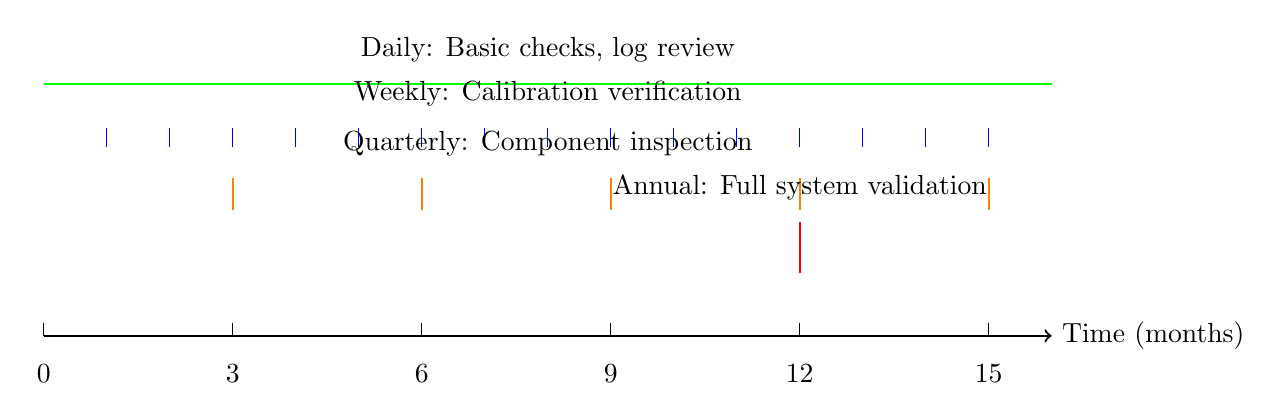
\begin{tikzpicture}[scale=0.8]
    % Maintenance timeline
    \draw[thick, ->] (0,0) -- (16,0) node[right] {Time (months)};
    
    % Daily tasks
    \draw[green, thick] (0,4) -- (16,4);
    \node[above] at (8,4.2) {Daily: Basic checks, log review};
    
    % Weekly tasks  
    \foreach \x in {1,2,3,...,15} {
        \draw[blue] (\x,3) -- (\x,3.3);
    }
    \node[above] at (8,3.5) {Weekly: Calibration verification};
    
    % Monthly tasks
    \foreach \x in {3,6,9,12,15} {
        \draw[orange, thick] (\x,2) -- (\x,2.5);
    }
    \node[above] at (8,2.7) {Quarterly: Component inspection};
    
    % Annual tasks
    \foreach \x in {12} {
        \draw[red, thick] (\x,1) -- (\x,1.8);
    }
    \node[above] at (12,2) {Annual: Full system validation};
    
    % Time markers
    \foreach \x/\label in {0/0, 3/3, 6/6, 9/9, 12/12, 15/15} {
        \draw (\x,0) -- (\x,0.2);
        \node[below] at (\x,-0.3) {\label};
    }
    
\end{tikzpicture}
\caption{Preventive Maintenance Schedule}
\label{fig:app-maintenance-schedule}
\end{figure}

This comprehensive installation and deployment guide ensures proper setup and commissioning of the RUS system, providing the foundation for safe and effective operation in clinical environments.
